%% \startreport{A/B Statistics}
%% \reportauthor{Some Jokers}
\documentclass[12pt]{report}
\usepackage{hyperref}
\usepackage{amsmath}
\usepackage{graphicx}
\newcommand{\be}{\begin{enumerate}} %% same as ramesh_abbr
\newcommand{\ee}{\end{enumerate}} %% same as ramesh_abbr
\newcommand{\beq}{\begin{equation}} %% new, no conflict
\newcommand{\eeq}{\end{equation}} %% new, no conflict
\newcommand{\bdm}{\begin{displaymath}} %% new, no conflict
\newcommand{\edm}{\end{displaymath}} %% new, no conflict
\newcommand{\bi}{\begin{itemize}} %% same as ramesh_abbr
\newcommand{\ei}{\end{itemize}} %% same as ramesh_abbr
\newcommand{\TBC}{\framebox{\textbf{TO BE COMPLETED}}} %% same as ramesh_abbr
\newcommand{\reals}{{\rm I\! R}} %% new, no conflict
\newcommand{\comp}[1]{\widetilde{#1}} 

%% From https://math.berkeley.edu/~gbergman/misc/hacks/langl_rangl.html
\newcommand{\langl}{\begin{picture}(4.5,7)
\put(1.1,2.5){\rotatebox{60}{\line(1,0){5.5}}}
\put(1.1,2.5){\rotatebox{300}{\line(1,0){5.5}}}
\end{picture}}

\newcommand{\rangl}{\begin{picture}(4.5,7)
\put(.9,2.5){\rotatebox{120}{\line(1,0){5.5}}}
\put(.9,2.5){\rotatebox{240}{\line(1,0){5.5}}}
\end{picture}}

\newcommand{\mymean}[1]{\ensuremath{\langl{#1}\rangl}} %% new, no conflict

\begin{document}

\title{A or B? A Bayesian Approach for Binary outcome tests}
\author{Ramesh Subramonian, Ranjeet S. Tate, Michael Shire, Abhinava Singh}
\date{}
\maketitle

\section{Introduction\label{sec:Intro}}

Consider the following \(A/B\) test. We direct users to one of two pages
-variants of the test- \(A\) and \(B\). On each page, there is an
action \(C\) that can be performed, called the {\em goal}. If a user
performs the goal (the trial is a {\em success}) it is equivalent to a
trial where a coin was tossed and observed to come up
Heads. (Subsequent visits by the user to that page are ignored, i.e.,
they are not counted as trials.) A user who visits the page and leaves
the page without performing the goal or never performs the goal
(within some time limit) is equivalent to a trial where a coin was
tossed and observed to come up Tails. The outcomes of such a trial are
binary valued: a success counts as a 1 and a trial without success
counts as 0.

We assume that there are some intrinsic or true probabilities of
success for Pages \(A\) and \(B\) ---\(p_A, p_B\) respectively--- which
are properties of the population. However, any finite experiment will
only yield results for a fraction of the population, a
{\em sample}. From the resulting experimental data for the sample we
want to induce the properties of the population on which to base decisions comparing \(A\) to \(B\).

As an example, let's say you are betting on the outcome of a coin
toss.  After a few tosses, you note that you seem to lose ``much more
often than random chance would have it''. How do we quantify this? If
you are basing your suspicion on 6 losses out of 10, you don't have
much reason to suspect the coin is loaded since even a fair coin will
yield that result quite often.  However, what if you lose 57 out a 100
times, or 550 out of a 1000 times?  We are interested in calculating
or estimating the true property of the coin based on its measured
behavior, or posterior to the experiment. In addition, we want to be
reasonably certain about this before acting on it by deciding not to
continue with the game or before accusing your possibly gun-toting
opponent of cheating.

Our knowledge of the induced properties is going to be
probabilistic. In the first example above, we think it more likely
that the coin has an intrinsic probability of 0.6 than of either 0.7
or 0.5. Conceptually, our knowledge of the intrinsic property will be
a probability distribution.

For the \(A/B\) test, once we have these estimates, as distributions
of \(p_A, p_B\), how do we use them to compare \(A\) and \(B\)?

At a very high level, our aim is
\begin{quote}
  to determine whether Page \(A\) is {\em significantly} (in a statistical
  sense) {\em better} than Page \(B\) in terms of the goal action, and
  whether the difference is {\em important} enough from a business
  perspective.
\end{quote}
For example, we may want to
know if \(p_A > p_B + \delta\) and with what confidence we claim that
to be true. Like our erstwhile POTUS with the verb ``to be'',
we will feel free to
define {\em significant}, {\em important} as well as {\em better}. 

\subsection{The Data Model}
As a result of the experiment, for each test-variant pair, we obtain
\bi
\item \(n_A, m_A\) --- the number, respectively, of trials and
  successes on Page \(A\)
\item \(n_B, m_B\) --- the number, respectively, of trials and
  successes  on Page \(B\)
\ei

\subsection{Components of the Problem}
How do we use this data to help us make decisions?
\be
\item First, the test owners (or we) have to establish a level at
  which the difference between the outcomes of \(A\) and \(B\) is
  important enough to be actionable. As a part of this process, we will choose a
  metric \(M\) by which to compare Page \(A\) and Page \(B\). For clarification, note that the choice of comparison metric is an issue that
  arises {\em only} when we want to quantify the comparison. If we
  were only interested in {\em whether} Page \(A\) is better than Page
  \(B\) then any metric (as long as it is monotonic in \(p_A\) and
  \(p_B\)) will do. The choice of metric becomes important when we are
  interested not just in whether Page \(A\) is better than Page \(B\),
  but in addition, {\em by how much}.
\item Second, we also have to decide on a credibility (or range of
  credibilities) associated with different business actions. We have
  to do this {\em before} beginning the experiment so we don't become
  vested in a positive outcome and allow ourselves to get carried away
  by serendipitous outcomes.
\ee

Once we have chosen a metric, there are two technical parts to this
problem:
\be
\item Using this data we have to calculate the posterior distribution
  of \(p_A, p_B\).
\item Then we have to use this distribution to calculate the
  relationship between the importance level and the credibility for
  the chosen metric.
\ee

\subsection{Outline}
We will start with describing in more detail what we mean by importance
level and credibility. Before analysing the results of the A/B test, we will
construct the posterior distribution of probabilities
for a single variant or page, and some useful properties of this
one-dimensional distribution. Then we will show how to calculate the
credibility for any metric \(M\) for comparing two variants. Once we have this
general result, we will propose and critically
analyse three different metrics for the comparison. Finally, for each of
these three metrics, we will calculate plots of importance level vs.
credibility for a sample outcome for \(n_A, m_A, n_B, m_B\).

\section{Importance Level and Credibility of the Results}
First, rewriting the above metric for ``better'' as \(p_A - (p_B +
\delta) > 0\), we see that we can generalize the question of ``better''
to whether
\(M(p_A, p_B)>0\) for some metric \(M\) which is a function on
the two-dimensional probability space \(p_A, p_B\).

Now, let's keep in mind that the question is not so much whether the
sample {\em behaved} better, i.e. whether
\(M(\frac{m_A}{n_A}, \frac{m_B}{n_B})>0\) for the mean probabilities of
success for the experiment, as it is
whether -based on the above data- there is a large likelihood that
the {\em true property of the population is better}.
If, from the data, we can induce the posterior
distribution for \(p_A, p_B\), the true success rates,
then we want to know the {\it credibility } or
probability \(P[M(p_A, p_B)>0]\) that \(A\) is better than \(B\) by an
important enough difference in terms of
metric \(M\). Both the metric \(M\) and the importance level are to be
established based on business considerations. Once a metric \(M\) has
been chosen and an importance level established, we want to know the
credibility with we can claim that this is a property of the population.
One can choose to establish a minimum credibiltity as well as a minimum
importance level to accept the proposition that A is better than B.

Of course, as the threshold difference increases, the credibility will
reduce: it is much more likely that a coin has a true 60\% or more probability
of landing Heads than it is that the coin has a true 80\% or more probability of
landing Heads, regardless of the experimental outcome.


\section{Bayesian Posterior Probability in One Dimension\label{sec:Bayesian1D}}
Consider the results for any one page, where we've made \(n\) trials
and obtained \(m\) successes.  The data corresponds to a distribution
with \(m\) 1s and \((n-m)\) 0s. The mean of this distribution, the
mean success rate, is \(\mu = m/n\) and the standard deviation of the
distribution is \(\sqrt{\mu\cdot (1-\mu)}\). The Standard Error in the
mean is
\bdm
  SE(\mu) = \sqrt{\frac{\mu\cdot(1-\mu)}{n}}
\edm
This is the experimental distribution, and the above values are used
in a Frequentist approach to calculating whether A is better than B,
see Sec.\ref{sec:frequentist} for more details.

Let \(X = x\) be the event that the
true property for that page is \(x\) (as opposed to it being any other
\(x'\neq x\)), in the distributional sense. Note that for this simple A/B test,
the true property is also a probability, so \(\{X\}=I\), the unit interval. 
If, as is the case, \(x\) is continuous, the probability that the true property
\(\in(x, x+dx)\) for some infinitesimal \(dx\) is given by
\bdm
P[X\in (x, x+dx)] = f(x)\cdot dx
\edm
where
\(f(x)\) is a probability distribution on \(\{X\}\). We
want to calculate \(f(x|n,m)\). There is no real way of knowing it or
deriving it without further assumptions, and we will take a Bayesian
approach to calculate it. Note that this is an assumption, and that
there are other approaches to calculating \(f(x|n,m)\) or \(P[M(x)>0]\),
frequently a frequentist approach or via simulations.


\subsection{Bayes' Theorem}

The Bayesian approach: Consider a ``scattering'' problem: for an
experiment, given prior knowledge of
the system, it is relatively easy to calculate the
probability distribution of the outcomes. For example, if we are given
a fair coin or other random element which has a mean probability of
50\% of turning up Heads and we conduct an experiment with \(n\)
trials, we can calculate the probability amplitude of getting \(m\)
Heads. Due to the mutually exclusive and collectively exhaustive
nature of the possible outcomes \(\{m\}\), we can normalize the
amplitudes and obtain a probability distribution over \(\{m\}\). This
can be generalized to a random element with any known mean probability
\(x\), yielding the Binomial distribution.
\bdm
P(m|x,n)={n \choose m}x^m (1-x)^{(n-m)}
\edm
which is normalized:
\bdm
\sum_{m\in[0,n]} P(m|x,n) = 1
\edm

The ``back-scattering'' or posterior problem is the reverse: In an experiment
of \(n\) trials with a coin or random element with {\it unknown}
probability \(x\), given that we obtained \(m\) Heads, what can we
conclude in a distributional sense about \(x\), a property of the
coin? Clearly, it is possible for any loaded coin with any finite true
probability \(x\) to yield exactly say 65 Heads out of 534 trials. Can
we be more quantitative and compute a probability distribution over
\(\{x\}\)?
\bdm
f(x|n,m)
\edm

The Bayesian approach is basically to say that we can calculate the
{\it amplitude} for any \(p\) to yield \(m\) successes out of \(n\)
trials as before, but now we fix \(n,m\) and use mutual exclusivity
and collective exhaustivity of the set of all \(x\), \(X =\{x\}\), to
normalize the {\it same} Binomial amplitudes to a probability
distribution over \(X\).   

In order to weight the amplitudes relatively before normalization, we
will use Bayes' Theorem.

Note that
\beq
P(X\cap Y)=P(X|Y)\cdot P(Y) = P(Y|X) \cdot P(X)
\eeq
is simply the requirement that the two different ways of calculating
the same joint
probability of \(X\) and \(Y\) yield the same result. This can be re-written
as Bayes'
Theorem, reproduced for convenience in Equation~\ref{eq:Bayes_Theorem}
\beq
\label{eq:Bayes_Theorem}
P(X|Y) = \frac{P(Y|X) \cdot P(X)}{P(Y)}
\eeq

\subsection{Derivation of the Posterior Probability Distribution for One dimension}
Let \(Y = m\) be the observed number of successes for a single variant with
\(n\) trials. Note that the number of trials
\(n\) is deterministic. Applying Bayes' Theorem, we want to calculate
\beq\label{eq:bayesapplied}
f(x|n,m) = \frac{P(m|x,n)\cdot P(x)}{P(m)}
\eeq
where we've identified \(f(x|n,m)\) with \(P(x|n,m)\).
Consider the three terms on the right hand side
\bi
\item 
Given that we have no prior knowledge of the true probability,
\(P(x)\) is assumed to come from the uniform distribution \(P(x)
=1\). With the goal of understanding a future term, note that the mean
probability for the uniform distribution is \(\frac{1}{2}\).
\item From the Binomial theorem, \(P(m|x, n) ={n \choose m}x^m
  (1-x)^{n-m}\)
\item 
\(P(m)\) is ill-defined but it can be absorbed into the normalization term
since we are
interested in normalizing the distribution \(f(x|n,m)\) over \(X\) and
the normalization term will be some function of \((n,m)\) such that
\bdm
\int_{x\in X}dx \cdot f(x|n,m) = 1
\edm
The distribution \(f(x|n,m)\propto x^m(1-x)^{n-m}\) can be recognized as the
beta distribution
\url{https://en.wikipedia.org/wiki/Beta_distribution} and
the normalization term can be looked up in
\url{https://en.wikipedia.org/wiki/Beta_fucntion#properties}.
\bdm
f(x|n,m) =\beta(x|m+1, n-m+1) = (n+1) {n\choose m}x^m (1-x)^{n-m}
\edm
\ei
which is the desired probability density that the population
probability of success is \(x\) given the sample outcome of \(m\)
successes from \(n\) trials. Note the ``extra'' normalization term \((n+1)\)
of the beta distribution on the unit interval
compared to the Binomial distribution on \(m\in[0,n]\)

\subsection{Properties of the Beta Distribution}
The Bayesian distribution of the posterior probabilities is a beta
distribution whose properties are well known.
\bi
\item The domain of the beta distribution is the unit interval  \(I =
  [0,1]\), and the beta distribution is 0 at \(x=0,1\)  for all \(n,m
  >0\).
\item The distribution is normalized over \(I\):
  \bdm
  \int_0^1 dx\cdot f(x|n,m) = 1
  \edm
\item The mode, or the value of x at which the distribution is a
  maximum, is given by
  \bdm
  {\tt mode}(x) = {\tt argmax}(\beta(x|m+1, n-m+1)) = \frac{m}{n}
  \edm
  Hence we hear the statement that the Bayesian posterior
  distribution is the ``maximum likelihood estimator''.
\item From the properties of the beta distribution,
the mean of the Bayesian distribution,
  \bdm \mu = \int_0^1 dx \cdot x\cdot f(x|n,m) = \frac{m+1}{n+2}
  \edm
  Note first that this is not
  equal to the mode, in fact the mean regresses from the mode towards
  0.5, which, in
  the absence of other information is the mean probability of the
  outcome of a binary valued experiment.
  Further, compare this mean of the posterior probabilities to the
  mean of the experimental distribution \(\frac{m}{n}\). This is
  effectively like adding a prior of \(50\%\) corresponding to
  one success and two trials to the actual experimental outcome.
  (This is the sophisticated Bayesian approach that Fox news
  takes: since "we don't know" and there are "two sides" to climate
  change, opinion is "balanced" by having one climate change denier
  for every climatologist.) Adding a "prior" is an
  effective way of reducing the noise in low outcome experiments. 
\item The beta distribution is not symmetric about the mean,
  except for the special case \(a=b\), in which case \(\mu = 0.5\):
  \bdm
  \beta(x|a,b) = \beta(2*\mu-x|a,b) \iff a=b
  \edm
\item The variance of the distribution is 
  \bdm
  \sigma^2 = var(x) = \frac{\mu\cdot(1-\mu)}{n+3}
  \edm
\item Since we've calculated the mean and the variance, we can
  approximate the Bayesian distribution by a normal distribution with
  the same mean \(\mu\) and variance \(\sigma^2\). These are
  {\it not} the mean and variance of the binary valued distribution of
  the outcomes of the experiment. Note further that the normal
  distribution has support
  outside the unit interval, is finite at the bounds of the interval
  and is symmetric about the mean, unlike the beta distribution it is
  meant to approximate.
\item The beta probability distribution, its
cumulative function 
  \bdm
  \beta_{cf}(x|a,b) = \int_0^{x'}dx'\cdot\beta(x'|a,b)
  \edm
  and its quantile function (the inverse of the cumulative function)
  are known in ``closed form'' as special functions in SciPy.
  \item in 
\ei

\section{Bayesian Approach to Comparing results of A/B test}\label{sec:bayesianab}
Given that user behavior on page \(A\) is independent of user behavior on
page \(B\), we
can create the joint probability density \(f(x, y)\), where \(x, y \in
I^2\) are the true probabilities \(x=p_A,y=p_B\)of Pages \(A\) and \(B\)
respectively.
\beq
\begin{split}
f_A(x)=f(x|n_A,m_A) &= \beta(x|m_A+1, n_A-m_A+1)\\ f_B(y)=f(y|n_B,m_B)
&= \beta(y|m_B+1, n_B-m_B+1)
\end{split}
\eeq
and
\bdm
f(x,y) = f_A(x)\cdot f_B(y)
\edm

Note that
\beq\label{eq:norm}
\int_{x=0}^{x=1} dx\int_{y=0}^{y=1} dy \cdot f(x, y) = 1
\eeq

Therefore, given a choice of comparison metric \(M\),
the probability that Page \(A\) is
``better'' in terms of metric \(M\) than Page \(B\) is 
\bdm
\int_{M(x,y)>0}dx \wedge dy \cdot f(x, y) \edm which is the \(f\)-weighted
area under the curve \(M(x,y) = 0\)

Let us solve \(M(x,y) = 0\) for \(y=M(x)\) (using the same notation
since it refers to the same curve), such that \(M(x,y) > 0\)
corresponds to \(y<M(x)\).  Then the double integral can be reduced to
\beq
\begin{split}
  P[M(p_A, p_B)>0] &= \int_{M(x,y)>0}dx \wedge dy \cdot f(x, y)\\
  &=
  \int_0^1dx\cdot \beta(x,m_A+1, n_A-m_A+1)\cdot\\
  &\beta_{cf}(M(x), m_B+1, n_B-m_B+1)
\end{split}
\eeq
where
\beq
\beta_{cf}(M(x), m_B+1, n_B-m_B+1)=
\int_0^{y=M(x)}dy'\beta(y',m_B+1, n_B-m_B+1)
\eeq
is the cumulative function of the beta distribution evaluated at \(M(x)\).

\section{Choice of Metric: What do we mean by ``better"?}\label{sec:metrics}
As before, let \(x= p_A = p(C|A)\) and \(y= p_B = p(C|B)\) be the underlying true probabilities for the event \(C\) to occur after the user lands on 
pages \(A\) and \(B\) respectively.
 
\subsection{Probability Difference}\label{sec:pdiff}
The most obvious metric on which to base the claim that \(A\) is
better than \(B\) is the difference \bdm M(x,y) = x-y >0 \edm If we
want to introduce the notion of a ``large enough" or important
difference, we can ask that \(x\) exceed \(y\) by a minimum amount
\(\delta\): \bdm M(x,y) = x-(y+\delta) >0 \edm What are the problems
with this metric?
\be
\item First, algebraically, even though probabilities
look like ``numbers'', they aren't real numbers; they belong to the
finite interval which does not have a natural affine structure, which
is a fancy way of saying that the difference between probabilities
isn't defined.
\item Second, from a geometric point of view, think of addition or
subtraction as taking steps on probability space. Then, depending on where you start, taking a finite
step causes you to fall off the edge. A somewhat fancier way of saying this is that under the metric
(\(ds^2 = dx^2\)),
probability space is geodesically incomplete. 
\item A third problem is that the notion of ``importance" is tied to the
results obtained. Assume that there is some monetary gain associated
with an increased success rate. One can translate the business
requirement into a minimum increase in the mean probability,
say by 0.1. This sounds
reasonable, since we are getting an additional 10\% of the population
to convert in the test variant \(A\) than we would in the control
variant \(B\). However, if the mean probability
for the control was small, say only 0.01, it would be completely
unreasonable to expect a test to raise that by 0.1 from 0.01 to 0.11. On the
other hand if we choose a smaller threshold for improvement, say 0.01,
for a large mean control success rate to increase from 0.50 to 0.51 doesn't
seem that important.
\ee

\subsection{Probability Lift}\label{sec:plift}
One way around the third problem listed above
would be to set a minimum threshold increase in terms
relative to the property of the control. After all, if the control were
projected to yield \(\$B\)
and the test to yield \(\$A\), it is reasonable to ask for a 10\%
increase in yield. This would translate into the lift metric
\bdm
M(x,y) = x-y*(1+\lambda) >0
\edm

Very often, this is rewritten to calculate the lift
\bdm
\lambda = \frac{x-y}{y}
\edm
The problem here, in addition to the first two problems from the previous section Sec.\ref{sec:pdiff}, is that we are dividing the difference of two probabilities
by a probability and these are not well defined operations on
probability space. If \(y\) happens to be small (which can happen if
the control group is improperly chosen) extremely large lift values
can result, which almost never extend to the population as a
whole. If one looks at the propagation of errors, the
lift is extremely sensitive to error in \(y\). If \(y\) is small and hence likely to be based on few successes, the relative variance \(var(y)/\mymean{y}\) is going to be large. This will be reflected in the variance of the lift, but magnified by a factor of \(\frac{x}{y^2}\). 

From a business perspective, there is another failing with this metric.
Consider a situation in which the success rate doubles from 0.05 to 0.10,
yielding a lift of 100\%. Now compare this with a situation in which the
success rate increased from 0.90 to 0.95. In terms of lift this appears to be
a paltry 5.6\%, and not very important. However, there are a couple of senses
in which this increase is just as important as from 0.05 to 0.10. First,
consider that if the control group success rate is 0.90 and we increase it
to 0.95, we've done half as well as we could possibly have: the maximum
possible improvement is by 0.10. On the other hand, when
we improved the success rate from
0.05 to 0.10, there was a lot of room for improvement (0.95), and we only
improved 0.05/0.95. Typically we deal with real numbers and it is enough to
consider how much we've improved by and ignore how much better we could have
done. Again, the problem with this metric is that we are
treating probabilities like real numbers and we are not taking into account
that probability space is bounded.

The lift metric also fails the test of ``universality'': Can one establish a
minimum importance level {\em before}
we know what the test results are? While we
can require a minimum lift of 100\% when the control group's success rate
is 0.05,, if the control group's success rate is already a high 0.9,
the maximum lift we can aspire to is 11.1\%.

Yet another way of looking at it is that we while we are taking the benefit of
being right into account (which is proportional to \(x\),
we are not taking into account the cost of being wrong, which is
proportional to \((1-x)\).

\subsection{Criteria for a Comparison Metric}\label{sec:criteria}
The biggest problem with the two metrics we've described so far is
that there is no clear question for which \(M(x,y) = x-y-\delta\) is the
answer. Let's drop for a moment the issue of the statistics and step back and consider the test situation: we have a
trial for a target event \(C\) that takes place under two separate
(sets of) conditions \(A\) and \(B\). From the data collected we
calculate or estimate \(x=p(C|A)\) and \(y=p(C|B)\) for the
population. Then we set about calculating
\(x-y-\delta\), but it is not clear that this metric is
associated with any logical proposition based on events and conditions
\(C,A,B\).

\subsubsection{What question does the difference metric answer?}
``Is \(A\) better than \(B\) as far as target \(C\) is concerned?''

If we are interested only in knowing whether ``\(A\) is better than
\(B\)'' (\(\delta = 0\), then we can calculate \(x-y\) or the
associated probability \(P(x-y)\) since it is both well-defined and
independent of metric or coordinate transformation. Probability space
does have an order and this order is independent of the specific
metric, i.e. for a function \(f\) which is monotonic in its arguments
\(x-y>0 \Leftrightarrow f(x,y) >0\) and \(P(x-y>0) = P(f(x,y) >
0)\). However, the moment we try to quantify this difference we run
into trouble. Suppose our proposition was ``If we were to run \(A\)
instead of \(B\) on \(U\) trials would we get more than a minumum
number of extra conversions?'' we are evaluating \(U*x - U*y -\Delta
U\) or \(x-y - \delta\) and we run into the problems already discussed
above.

Are \(A\) and \(B\) independent channels for the target
action \(C\)? For example the control \(B\) may be a set of available clicks and
\(A\) may represent a page with an {\em additional} available click. Let's say that the click probability increased\(x>y\). Are
we then trying to find the probability associated with a page which
would have just the one available click, which conceptually might look like \(\frac{x-y}{1-y}\)? Are we trying to calculate something
like \(p(C|A\cap \comp{B})\)? But this makes no sense if \(A\) and \(B\)
are disjoint!

Contrast this approach with how we develop the combined odds: There we know the probability of C under two independent (but not disjoint) conditions A and B, \(P(C|A)\) abd \(P(C|B)\) (see combined odds for a full discussion). We have two numbers and we could just start adding them and multiplying them or taking the geometric mean because we guess that that captures what happens when A and B co-occur. Instead, we first fomulate a definite proposition: what is the probability of C given both A and B occur. {\em Then} we try to derive the answer. We could have failed to derive the answer or there may be alternate answers, but at least the question is defined \(p(C|A\cap B)\).

AS far A/B testing goes, there are plenty of distance funcrtions \(d(x,y)\) on probability space based on information, theory, quantum theory and thermodynamics. What do any of them have to do with a business goal?
So the main lesson here is to {\em not} start analysis (perhaps not even the experiment) until a clrearly defined business or logical proposition is at hand. This propositon will define the comparison metric and we can proceed along the lines in Sec. ... 

The metric should arise from a clearly defined business or logical proposition.

In the absence of a logical or business propsition, based on the dissatisfactions with the above metrics, we can
establish the following criteria a good metric should satisfy:
\bi
  \item The metric should be familiar to non-technical people.
  \item The metric should be universal in the sense that a threshold
    value can be decided on {\em without} knowing in advance the
    results of the experiment for the control group.
  \item It should be based on sound mathematical principles.
  \item The metric should be invariant under the discrete symmetry
\bdm
(n_A, m_A, n_B, m_B) = (n_B, n_B - m_B, n_A, n_A - m_A)
\edm
i.e., the conditions under which ``A is better than B'' (A has more wins than B)
should be the same as the conditions under which ``B is worse than A''
(B has more losses than A).
\ei

\subsection{Odds factor}\label{sec:oddsfactor}
For a probability \(p\), the {\em odds} are \(p:(1-p)\), or
\beq\label{eq:oddsp}
o(p)=\frac{p}{1-p}
\eeq
From the odds, the probability can be recovered by
\beq\label{eq:podds}
p(o) = \frac{o}{1+o}
\eeq

Why do gamblers think in terms of odds rather than probabilities? One suspects
because they intuitively understand that when evaluating a position
they have to take into account the cost of failure \$\(C\) as well as the
benefits of success \$\(B\) and they are evaluating and optimizing the
{\it benefit-to-cost-ratio}
\bdm
\frac{\$B \cdot p}{\$C \cdot (1-p)}
\edm
Since both \$\(B\) and \$\(C\) are presumed constant, they drop out of
consideration and one wants to increase the odds.
So to compare the results of \(A\) and \(B\) one metric we could be looking at
is
\beq
\label{eq:oddsfactor}
M(x,y) = \frac{o(x)}{\phi o(y)} -1 = \frac{x/(1-x)}{\phi\cdot y/(1-y)}-1
\eeq
This is interpreted as saying that the odds associated with \(A\) are at
least \(\phi \times\) the odds associated with \(B\).

In the absence of a clear business proposition (as one has with the
mean page-visits metric in Sec.s\ref{sec:vdiff} and \ref{sec:vlift},
the above metric accounts for the existence of a finite cost of
failure as well as the benefit of success, {\em without knowledge of
  the actual values of the benefit or cost}. \footnote{In contrast, an
  additive approach like \(\$B\cdot x - \$C\cdot(1-x)\) requires us to
  know at least the {\em ratio} of benefit to cost.}  Furthermore, it
is familiar to gamblers, bookies, fixers, other degenerates as well as
normal people who visit Las Vegas.

Before we consider the last two criteria, let us introduce the
{\it logit coordinate}
corresponding to a probability \(p\)
\bdm
\omega = \log(\frac{p}{(1-p)})
\edm
which belongs to \(\reals=(-\infty, \infty)\). Note that this is the
inverse of the logistic function
\bdm
p=\frac{1}{1+e^{-\omega}}
\edm

On \(\reals\)
we also know how to do algebra, we can
add or subtract without fear of falling off the edge, as well as multiply
and divide. In particular we can add a scalar, so we can take differences,
not in probability space, but in logit space:
\bdm
M(x,y) = \omega(x) -(\omega(y) + \log(\phi))
\edm
which is the same criterion as in Eq. \ref{eq:oddsfactor}.
Note that this action is mathematically sound and there are no restrictions on
the choice of \(\phi\) based on the values of \(x\) or \(y\).

For different values of \(\phi\), in 2D probability space this metric
defines a family of curves from \(O\) to the point \((1,1)\), bowed into the
lower right triangle as \(log(\phi)\) increases. For \(\phi=1\), this
reduces to the \(45^\circ\) line corresponding to the requirement that
\(x\) be greater than \(y\). 

For small values of \(x<<1\) and \(y<<1\), \(\phi-1\) is simply the lift in
the success rate \(p\). For values of \(x\) and \(y\) close to 1,
\(\phi-1\) is the
fractional drop in the failure rate \((1-p)\). The curves are symmetric under
reflection in the line \(x+y = 1\), i.e. under the transformation
\bdm
(x,y)\rightarrow (1-y,1-x)
\edm

As an aside, the normalization in Eq.\ref{eq:norm}
has been carried out assuming that the
line element on probability space is simply
\bdm
ds = dp
\edm
The metric this corresponds to is geodesically incomplete. A better line
element or metric on probability space can be pulled-back from logit space:
On \(\reals\) there is a
natural Euclidean metric
\bdm
ds^2 = d\omega^2
\edm
which we can pullback to probability space
\bdm
ds = d\omega = \frac{\partial \omega}{\partial p}dp = \frac{1}{p\cdot(1-p)}dp
\edm
and which we can potentially use to define and normalize distributions on
probability space.

\subsection{Page Visits Difference}\label{sec:vdiff}
For a website, define the {\em page transition probability} \(\tau\)
as the probability that a user on a page on the website moves to
another page on the website within a fixed amount of time, as opposed
to letting their session end or navigating off the site. Now imagine
an A/B test in which the page transition probability is measured for
users in two variants. While it is undeniable that increasing the page
transition probability is a good outcome, does the difference in
probabilities capture a business goal? A common (as in not-rare) goal
for many websites is to increase the ``stickiness'' of the website or
to increase the number of pages visited by a user during a session. On
average, the monetizability is linearly related to the mean number of
pages visited. So how is the average page visits \mymean{P} related to
the page transition probability \(\tau\)? Since it is generated from a Poisson process, the page visit histogram (rather, its cumulative function) is an exponential decay and 
\beq\label{eq:visitstau}
\mymean{P} = v(\tau) = \frac{1}{1-\tau}
\eeq
In terms of the mean page visits, the effective page transition probability is given by the inverse function
\beq\label{eq:tauvisits}
\tau(v) = 1-\frac{1}{v}
\eeq
See pageviewsanalysis.pdf for a detailed explanation.

So to compare the results of \(A\) and \(B\) the metric we should be looking at
is
\beq
\label{eq:visitsdiff}
M(x,y) = v(x) - v(y)-\Delta P
\eeq
This is interpreted as saying that the mean number of page visits associated with \(A\) increased over those associated with \(B\) by \(\Delta P\) pages.

Note that this action is mathematically sound and there are no restrictions on
the choice of \(\Delta P >0\) based on the values of \(x\) or \(y\).

\subsection{Page Visits Lift}\label{sec:vlift}
Alternately, we can compare the results of \(A\) and \(B\) relatively,
in which case the metric we should be looking at is
\beq
\label{eq:visitslift}
M(x,y) = v(x) - v(y)*(1+\delta P)
\eeq
This is interpreted as saying that the mean number of page visits
associated with \(A\) increased over those associated with B by a
factor \(\delta P\) pages.


\subsection{Comparison of the Metrics}
In order to get a better feeling for the metrics, for each of them,
let's look at the contour in 2D probability space for a fixed
threshold value. These are the boundaries we've calculated later, in
Sec.\ref{sec:boundaries}. First, let us look at the comparison metrics
for probability in Fig.\ref{fig:probmetrics},
\begin{figure}[ht!]
\centering
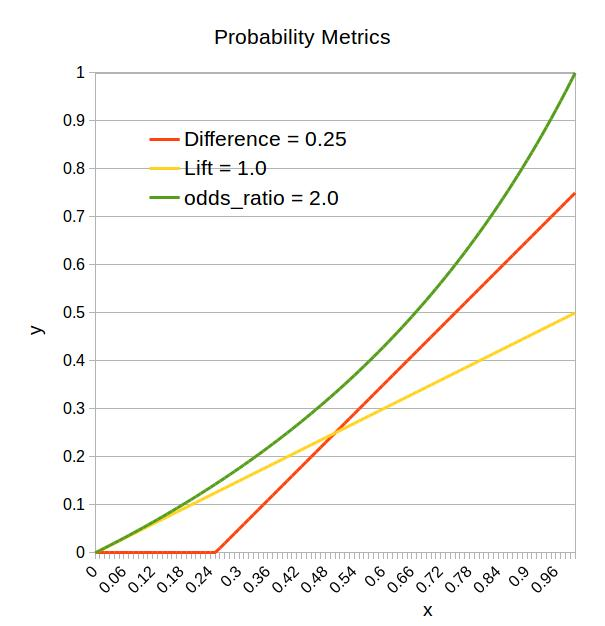
\includegraphics[width=90mm]{figures/probability_metrics}
\caption{Probability Comparison Metrics on 2D Probability
  space \label{fig:probmetrics}}
\end{figure}
where we see that both the difference metric and the lift are bounded
and do not apply to all values of \((x,y)\). The odds factor has no
such limitations.

Next, in Fig. \ref{fig:visitsmetrics}, we plot the difference and lift
comparison metrics for page visits.
\begin{figure}[ht!]
\centering
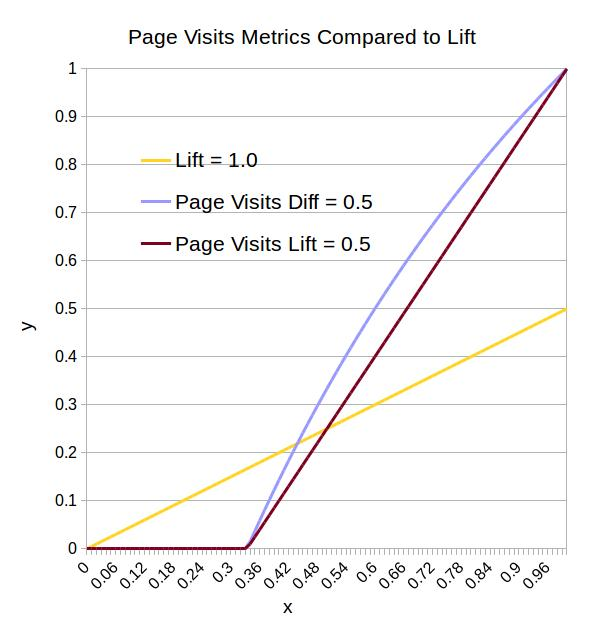
\includegraphics[width=90mm]{figures/page_visits_metrics}
\caption{Page Visits Comparison Metrics on 2D Probability
  space \label{fig:visitsmetrics}}
\end{figure}
For comparison, we've also plotted the probability lift
boundary. There are a few things to note.
\be
\item When their threshold values are 0, the boundaries for all 5
  metrics collapse to the \(45^\circ\) diagonal line, and all the
  Bayesian credibilities will be the same.
\item However, when the thresholds have non-zero values, the
  boundaries are {\em not} the same. As we can see in
  Fig.\ref{fig:visitsmetrics}, there is a large gap between the page
  visits metric boundary and the probability lift boundary, which
  means that for any joint probability distribution with significant
  support in one of those gaps the two metrics could potentially lead
  to contradictory decisions: If the joint probability distribution
  has support in the gap in the bottom left corner (\(x\) and \(y\)
  small and \(x>y\)), then the importance and statistical standard to
  decide in favor of varant \(A\) will be met based on the probability
  lift but not on the basis of the page views lift. The opposite will
  hold true if the joint probability distribution has significant
  support in the top right hand corner, where (\(x\) and \(y\) are
  both close to 1 and \(x>y\)).
\item Though the boundaries for both the page visits comparison
  metrics look very similar to each other for the same value of the
  threshold importance, the meaning of the threshold is very
  different: in one case it is the absolute increase in the average
  number of pages visited per session, and in the other case it is the
  \% increase. Of course these two measures will coincide when the
  average number of visits is 1 and they will coincide asymtotically
  as the number of page visits tends to infinity.
\item When the transition probability is very small in the control
  group (\(y\rightarrow 0\)), it takes a large increase in the test
  transition probability to effectuate a modest increase in the page
  visits. On the other hand, when the page transition probabiity is
  large (\(y\rightarrow 1\)), only a small increase in in transition
  probability is needed to see a large increase in the number of pages
  visited.
\ee

\section{Implementation Details}

\subsection{Boundaries for Integration of Bayesian Distribution}\label{sec:boundaries}
As we've seen in Sec.\ref{sec:bayesianab}, to calculate the Bayesian
credibility we integrate the Bayesian joint probability distribution
over the region that satisfies the threshold for the chosen
metric. Hence we have to represent the metric as a boundary in the 2D
probability space, by solving \(M(x,y,\delta) = 0\) for
\(y=M(x,\delta)\) for each metric \(M\) and corresponding threshold
\(\delta\). These are the boundaries or contours we've plotted in
Fig.\ref{fig:probmetrics}

\subsubsection{Boundary: Probability Difference}
The boundary is defined by
\beq
M(x,y,\delta) = x-(y+\delta) =0
\eeq
which is solved for
\beq
y=M(x,\delta) = x-\delta
\eeq

\subsubsection{Boundary: Probability Lift}
The boundary is defined by
\beq
M(x,y,\lambda) = x-(1+\lambda)*y =0
\eeq
which is solved for
\beq
y=M(x,\lambda) = \frac{x}{1+\lambda}
\eeq

\subsubsection{Boundary: Odds Factor}
The boundary is defined by
\beq
M(x,y,\phi) = o(x)-\phi *o(y) =0
\eeq
which is solved for
\beq
y=M(x,\phi) = p\left(\frac{o(x)}{\phi}\right)
\eeq

\subsubsection{Boundary: Page Visits Difference}
The boundary is defined by
\beq
M(x,y,\delta_v) = v(x)-(v(y)+\delta_v) =0
\eeq
which is solved for
\beq
y=M(x,\delta_v) = \tau(v(x)-\delta_v)
\eeq
where \(v(\tau)\) and \(\tau(v)\) are defined in Eq.s\ref{eq:visitstau} and \ref{eq:tauvisits} respectively. 

\subsubsection{Boundary: Page Visits Lift}
The boundary is defined by
\beq
M(x,y,\lambda_v) = v(x)-(1+\lambda_v)*v(y) =0
\eeq
which is solved for
\beq
y=M(x,\lambda_v) = \tau\left(\frac{v(x)}{1+\lambda_v}\right)
\eeq

\subsection{Integrating the Product of the Beta Distributions}
The Python package scipy.stats includes the \(\beta\) distribution
{\tt beta.pdf(p|a,b)} and its cumulative function {\tt beta.cdf(p|a,b)}. Very
significantly, the quantile function or the inverse of the cumulative function
{\tt beta.ppf(percentile|a,b)} -which allows one to calculate the values of
\(p\) at which a given percentile of the distribution occurs- is also
implemented.

Why is this important? For numerical plotting routines or for numerical
integration one discretizes the domain \(x\) into a set of points at which to
evaluate the beta distribution or its cumulative function.
For any number of points which break up the domain into uniform intervals,
there exists a number of trials \(n\) which is large enough that the effective
support of the beta distribution is smaller than an interval, resulting
in graphical or numerical integration errors which will exceed any given
tolerance. The graph will appear as a spike and the integral will be either 0
or some absurdly incorrect value.

So what can we do?
Assuming that we can tolerate an error of ~0.2\%, what we want to do
is integrate or plot over the subset of the domain with
some large proportion, say 99.8\% of the support. Then we can use
\({\tt beta.ppf}()\) to calculate the minimum and maximum values of
the discrete set as
\beq
\begin{split}
  x_{0.1\%}&={\tt beta.ppf(0.001|m+1, n-m+1)}\\
  x_{99.9\%}&={\tt beta.ppf(0.999|m+1, n-m+1)}  
\end{split}
\eeq
While one is again tempted to break up the subset \([x_{0.1\%},x_{99.9\%}]\)
into 998 uniform intervals,
in fact the thing to do is to break it up into smaller intervals where the
distribution is larger and vice versa. This corresponds to finding the
\(x-\)values for uniformly selected quantiles, we are effectively
discretizing the {\em range} of the cumulative function uniformly:
\bdm
{\tt Array(x)} = {\tt beta.ppf(Array([0.001, 0.999, step = 0.001])|m+1, n-m+1)}
\edm
Since ``(99.8\% of) everything'' is happening in this range of
\(x\) values, using this array for both plotting and numerical integration is
very robust.

\section{Sample results for Bayesian Credibility}
For test results with \((n_A, m_A, n_B, m_B) = (200, 40, 100, 15)\), we plot
the credibility as a function of the importance levels for the three metrics
proposed above.

\subsection{Probability Difference}
\begin{figure}[ht!]
\centering
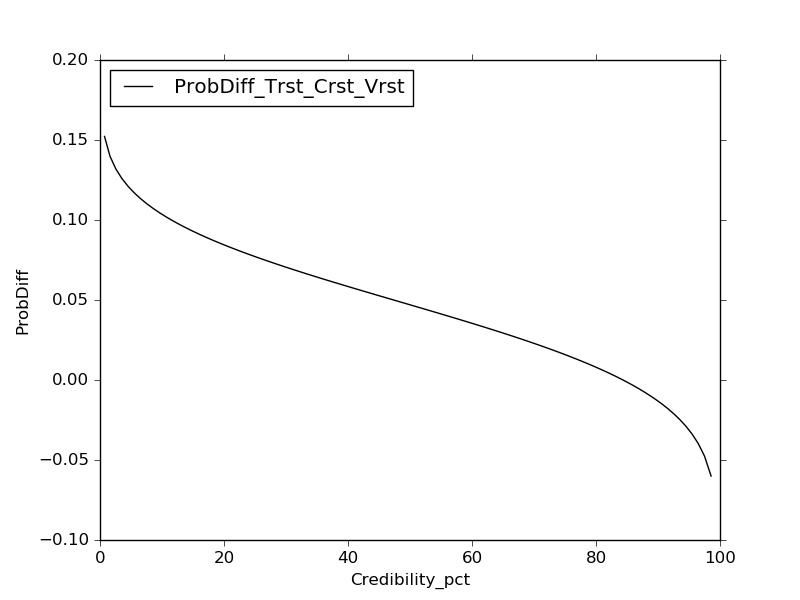
\includegraphics[width=90mm]{figures/ProbDiff_Trst_Crst_Vrst}
\caption{Delta vs. Credibility \label{fig:delta_vs_cred}}
\end{figure}
From Fig.  
\ref{fig:delta_vs_cred} the user can read-off the delta which
corresponds to a chosen credibility. We see
that as expected the credibility drops as the
threshold by which \(p_A\) should exceed \(p_B\) increases. The symmetry
discussed in Sec. \ref{sec:criteria} also holds for the difference
metric.

\subsection{Probability Lift}
\begin{figure}[ht!]
\centering
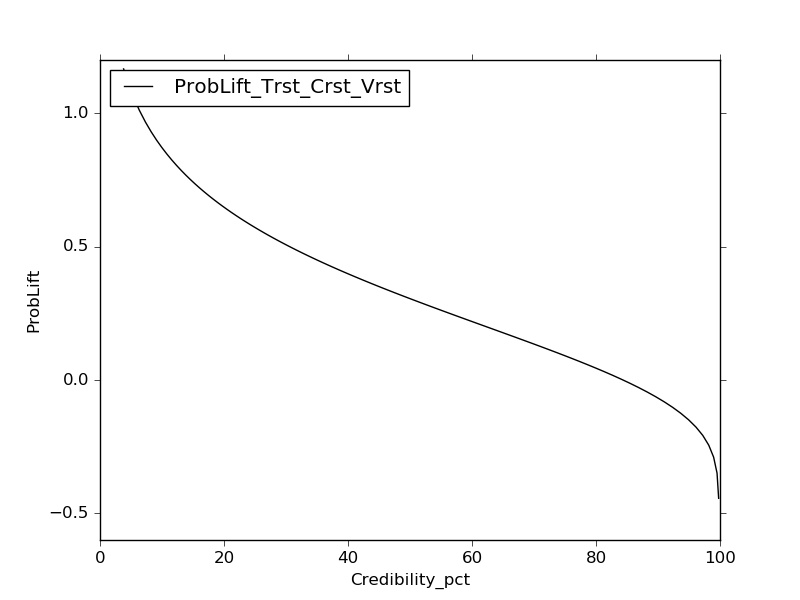
\includegraphics[width=90mm]{figures/ProbLift_Trst_Crst_Vrst}
\caption{Lift vs. Credibility \label{fig:lift_vs_cred}}
\end{figure}
From Fig.  
\ref{fig:lift_vs_cred} the user can read-off the lift which
corresponds to a chosen credibility. We see that as expected the
credibility drops as the lift threshold increases.

\subsection{Odds Factor\label{sec:odds-factor-result}}
\begin{figure}[ht!]
\centering
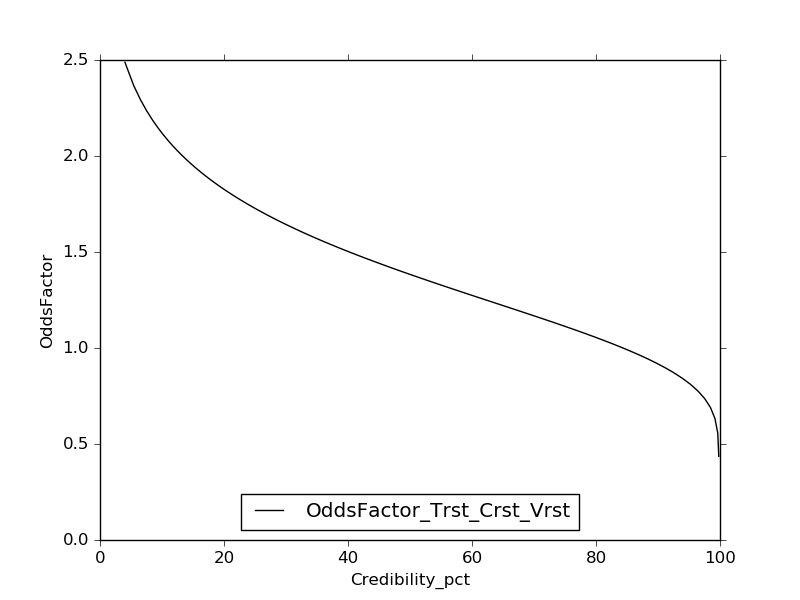
\includegraphics[width=90mm]{figures/OddsFactor_Trst_Crst_Vrst}
\caption{Odds factor vs. Credibility \label{fig:factor_vs_cred}}
\end{figure}
From  Fig.
\ref{fig:factor_vs_cred} the user can read-off the odds factor which
corresponds to a chosen credibility or vice versa. We see
that as expected the credibility drops as the
threshold by which \(odds_A\) should exceed \(odds_B\) increases.
We also point out that, due to the symmetries of the odds and
those of the beta distribution,
the Odds Factor vs. credibility curve is invariant under the discrete symmetry
\bdm
(n_A, m_A, n_B, m_B) = (n_B, n_B - m_B, n_A, n_A - m_A)
\edm
discussed in Sec. \ref{sec:criteria}.

\subsection{Page Visits Difference\label{sec:visits-diff-result}}
\begin{figure}[ht!]
\centering
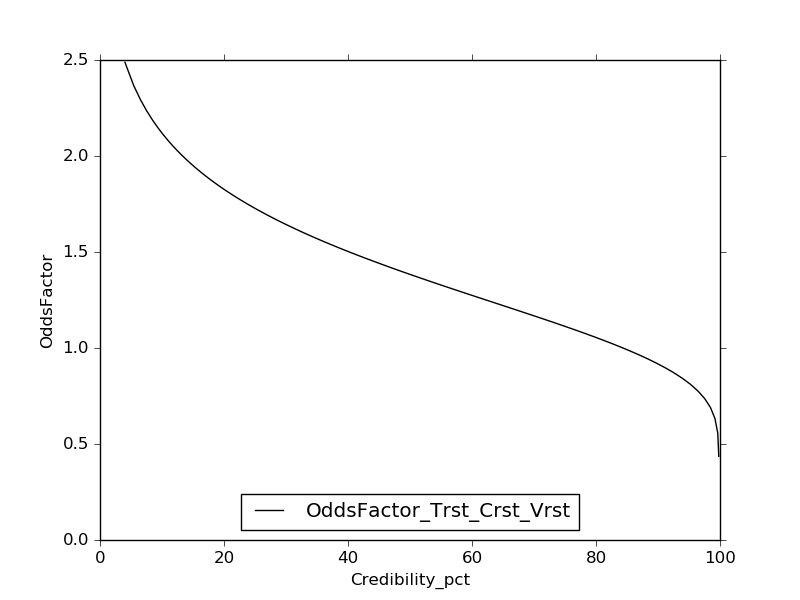
\includegraphics[width=90mm]{figures/OddsFactor_Trst_Crst_Vrst}
\caption{Difference in Page Visits vs. Credibility \label{fig:visitsdiff-vs-cred}}
\end{figure}
From  Fig.
\ref{fig:visitsdiff-vs-cred} the user can read-off the odds factor which
corresponds to a chosen credibility or vice versa. We see
that as expected the credibility drops as the
threshold by which \(v_A\) should exceed \(v_B\) increases.

\subsection{Page Visits Lift\label{sec:visits-lift-result}}
\begin{figure}[ht!]
\centering
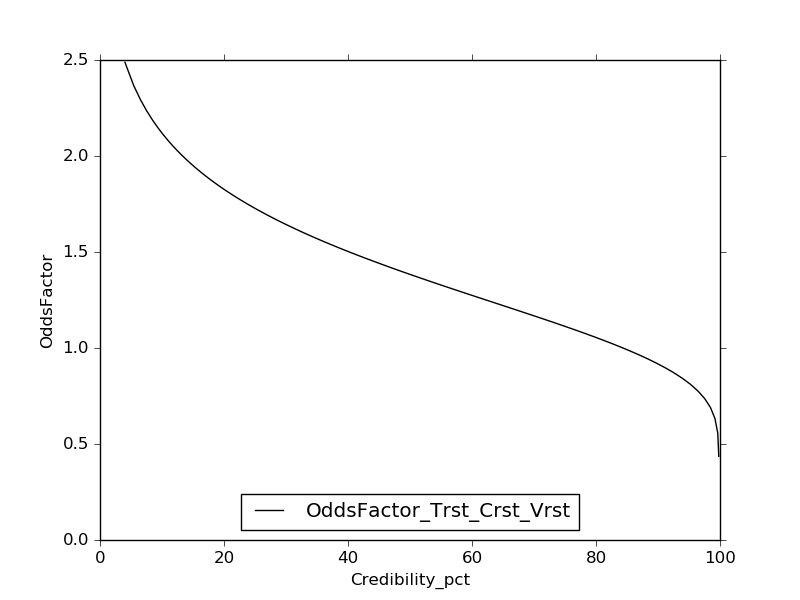
\includegraphics[width=90mm]{figures/OddsFactor_Trst_Crst_Vrst}
\caption{Page Visits Lift vs. Credibility \label{fig:visitslift-vs-cred}}
\end{figure}
From  Fig.
\ref{fig:visitslift-vs-cred} the user can read-off the odds factor which
corresponds to a chosen credibility or vice versa. We see
that as expected the credibility drops as the
threshold by which \(v_A\) should exceed \(v_B\) increases.

\section{The Standard Frequentist Approach\label{sec:frequentist}}
The material in this section is well-known and is included for completeness
and comparison. For an utterly convincing argument that demonstrates the
superiority of the Bayesian approach without assuming any {\em a priori}
knowledge of statistics, please take the time to read
\url{https://xkcd.com/1132/}.

\subsection{Single Variant}\label{sec:frequentist1D}
Consider the situation for one variant as described earlier in Section
\ref{sec:Bayesian1D}, with \(n\) trials indexed by \(i\) and the corresponding
outcomes \(x_i\in \{0,1\}\). Let there be \(m\) successes (\(1\))
and \(n-m\) failures (\(0\)). Then the mean or expectation of \(\{x_i\}\) is
\bdm
\mymean{x} = \mu = \frac{1}{n}\sum_i x_i = \frac{m}{n}
\edm
and the variance of the distribution is
\bdm
var(x) = \sigma^2_x = \mu\cdot(1-\mu)
\edm
where \(\sigma_x\) is the standard deviation.

The (Frequentist) mean of the distribution is considered a good estimate
of the mean of the population:
\bdm
\mu_F = \mu
\edm
Now, we are primarily interested in the variance or the
Standard Error in the estimated mean. From the definition of variance, it
is fairly easy to show that the variance of a linear combination of
{\em independent} stochastic variables is the sum of the squares of the
components:
\bdm
var(x+\alpha\cdot y) = var(x) + 2\alpha\cdot covar(x,y)+ \alpha^2\cdot var(y)
\edm
(Think of the SE as the \(L^2\) norm of the error vector under the covariance
metric.) Since the \(\{x_i\}\) are all independent, elementary algebra yields
that the variance of the mean is
\bdm
var(\mu) = var(\mymean{x}) = n\cdot\frac{var(x)}{n^2} =/
\frac{\mu\cdot(1-\mu)}{n}
\edm
and the Standard Error in the mean:
\bdm
\sigma_F = \sqrt{\frac{\mu\cdot(1-\mu)}{n}}
\edm
One then assumes that \(\mu\) is normally distributed and uses the
cumulative function of the Normal distribution with the above parameters to
calculate \(z\)-scores, percentiles or \(p\)-values.

\subsection{Mean and Variance of a Function of Stochastic Variables}
As before, let \(M(x,y,\delta)>0\) be the (1-sided) proposition we
want to test, where \(M\) is one of the comparison metrics defned in
Sec.\ref{sec:metrics}. If we had estimates for \mymean{M} and
\(SE(M)=\sqrt{var(M)}\) then we could calculate the \(z\)-statistic
for the proposition
\beq\label{eq:zstat}
z(M)= \frac{\mymean{M}}{SE(M)}
\eeq
and proceed to calculate the parametric confidence level or
\(p\)-value. Since at least some of the comparison metrics are not
linear in their arguments, it is possibly not as trivial to calculate
the mean and variance. The following are decent estimates.

Let \(X = \{x^i\}\) be a stochastic variable belonging to an
\(n-\)dimensional differentiable space. Let \(f(X)\) be a function on
this space\footnote{For the details of the derivation of these results
  see mean\_variance\_of\_function.pdf}.
\beq\label{eq:meanoff}
\mymean{f(X)} \approx f(\mymean{X}) + \frac{1}{2}covar(x^i,x^j)\cdot f_{0,ij}
\eeq
In the above approximation for the mean of a function, the first term
is the function of the mean. Consider the second term. The first
multiplicand is simply the covariance matrix for the variables
\(X\). The second multiplicand is the Hessian -the matrix of mixed
second partial derivatives- of \(f\) (evaluated at \(X=X_0\))
\beq
f_{0,ij} = \left. \frac{\partial}{\partial x^i}\frac{\partial}{\partial x^j}f(X)\right|_{X=X_0}
\eeq
is (the \(i,j-\)th component of) the second derivative of \(f\)
w.r.t. \(X\) evaluated at the point \(X=X_0\).  The two matrices are
multiplied and the trace is taken to produce a scalar.

The variance of the function is given by
\beq\label{eq:varoff}
var(f(X))\approx f_{0,i}\cdot covar(x^i,x^j)\cdot f_{0,j}
\eeq
where
\bdm
f_{0,i} = \left. \frac{\partial}{\partial x^i}f(X)\right|_{X= X_0}
\edm
is the \(i-\)th component of the gradient of \(f\) w.r.t. \(X\)
evaluated at the point \(X=X_0\).

\subsection{Calculating the Frequentist Credibilities at Default Thresholds}
For ease of reading we will repeat the metrics here and then present
the mean and variance for each. Note that \(x=p_A\) and \(y=p_B\) are
the probabilities for the two variants. The mean \mymean{x} and
variance of the mean \(var(\mymean{x})\) for each is calculated in the
beginning of this section. Since the two variants are disjoint, the
covariance \(covar(x,y)\) is 0.

\subsubsection{z: Probability Difference}
The proposition is
\beq
M(x,y,\delta) = x-(y+\delta) > 0
\eeq
from which
\beq
\begin{split}
  \mymean{M} &=\mymean{x} - \mymean{y} - \delta \\
  var(\mymean{M}) &= var(\mymean{x})+var(\mymean{y})
\end{split}
\eeq

\subsubsection{z: Probability Lift}
The proposition is
\beq
M(x,y,\lambda) = x-(1+\lambda)*y >0
\eeq
from which
\beq
\begin{split}
  \mymean{M} &=\mymean{x} - (1+\lambda)*\mymean{y} \\
  var(\mymean{M}) &= var(\mymean{x})+(1+\lambda)^2*var(\mymean{y})
\end{split}
\eeq

\subsubsection{z: Odds Factor}
The proposition is
\beq
M(x,y,\phi) = o(x)-\phi *o(y) >0
\eeq
From Eq.\ref{eq:oddsp}
\beq
\begin{split}
  \frac{do}{dx} &= \frac{1}{(1-x)^2} \\
  \frac{d^2o}{dx^2} &= \frac{2}{(1-x)^3}
\end{split}
\eeq
which can be substituted in Eq.s\ref{eq:meanoff} and \ref{eq:varoff} for
\beq
\begin{split}
  \mymean{M} &=o(\mymean{x}) + \frac{var(\mymean{x})}{(1-\mymean{x})^3} - \phi*\left(o(\mymean{y}) + \frac{var(\mymean{y})}{(1-\mymean{y})^3}\right) \\
  var(\mymean{M}) &= \frac{var(\mymean{x})}{(1-\mymean{x})^4} + \phi^2*\frac{var(\mymean{y})}{(1-\mymean{y})^4}
\end{split}
\eeq

\subsubsection{z: Page Visits Difference}
The proposition is
\beq
M(x,y,\delta_v) = v(x)-v(y)-\delta_v >0
\eeq
From Eq.\ref{eq:visitstau}
\beq
\begin{split}
  \frac{dv}{dx} &= \frac{1}{(1-x)^2} \\
  \frac{d^2v}{dx^2} &= \frac{2}{(1-x)^3}
\end{split}
\eeq
which can be substituted in Eq.s\ref{eq:meanoff} and \ref{eq:varoff} for
\beq
\begin{split}
  \mymean{M} &=v(\mymean{x}) + \frac{var(\mymean{x})}{(1-\mymean{x})^3} - v(\mymean{y}) - \frac{var(\mymean{y})}{(1-\mymean{y})^3} -\delta_v\\
  var(\mymean{M}) &= \frac{var(\mymean{x})}{(1-\mymean{x})^4} + \frac{var(\mymean{y})}{(1-\mymean{y})^4}
\end{split}
\eeq

\subsubsection{z: Page Visits Lift}
The proposition is
\beq
M(x,y,\lambda_v) = v(x)-(1+\lambda_v)*v(y) >0
\eeq
which can be re-written in linear form as
\beq
(1-y)-(1+\lambda_v)*(1-x) >0
\eeq
from which
\beq
\begin{split}
  \mymean{M} &=(1-\mymean{y}) - (1+\lambda_v)*(1- \mymean{x})\\
  var(\mymean{M}) &= var(\mymean{y})+(1+\lambda_v)^2*var(\mymean{x})
\end{split}
\eeq



\subsection{Comparing Bayesian and Frequentist percentiles for a single variant}
As we will show in a later post, the odds corresponding to
the percentiles calculated via the Frequentist+parametric approach
are within \(10\%\) of the Bayesian percentile odds if:
\beq
\begin{split}
  n &>\approx 100\\
 {\rm and } m &>\approx 20
\end{split}
\eeq
So of course, if we have ``lots'' of data the two approaches agree.
If we don't have even as
little data as required above, then the Bayesian approach,
which doesn't rely on the assumption of normality, is more reliable. But for
what? You are still going to have small confidence intervals or large
\(p\)-values, so only if you are in the business of ``0\(\sigma\)''
decision-making would you use the results from such a small sample. From a
statistical point of view, for small probability phenomena, the ``bigness of
data'' is determined by the number of positives, not the number of trials.

\subsection{Comparing Bayesian and Frequentist for Two Variants}
Analyzing the A/B situation described in the Introduction
\ref{sec:Intro}, we want to compare \(\mu^A_F\) to \(\mu^B_F\). If the
comparison metric is linear in both, as would be the case with the difference
or the lift, the distribution of the comparison metric is also normal, as long
as the conditions of applicability of the Central Limit Theorem still hold for
each variant. However, normality is {\em not} preserved under non-linear
transfornications, for example for the odds-factor metric discussed in
Sec. \ref{sec:oddsfactor}. 

The algebra based parametric approach has a further
problem in that it is {\em ill-defined}.
Consider the relatively simple Lift as a
comparison metric: The proposition is that \(p_A\) exceeds \(p_B\) by a
proportion \(\lambda\) of \(p_B\). This can be cast algebraically as
\bdm
{\rm M_{Lift1} }: p_A - (1+\lambda)\cdot p_B > 0
\edm
Since it is linear, there are no approximations involved in calculating
its mean and variance and hence \(z\). However, it can also be re-cast
algebraically as
\bdm
{\rm M_{Lift2} }: \frac{p_A}{p_B} - (1+\lambda) > 0
\edm
This is a non-linear function and approximations will be required to calculate
its mean and variance. The resulting \(z\) and credibility
will be different for the {\em same} proposition.

Both of the above algebraic metrics represent the same geometric object,
a curve in \((p_A, p_B)\) space. In the Bayesian approach, the proposition is
cast as the calculation of
the (weighted) area under this curve, and is manifestly independent of
algebraic transformations of the comparison metric.

We plan to discuss alternate approaches and a more
detailed comparison of parametric and non-parametric approaches in
future posts, where we will show that the credibility calculated via parametric approaches
can deviate very significantly from that calculated non-parametrically.

\section{Appendix}
\subsection{The Kullback-Leibler Probability Divergence as a metric on probability space}
Let \(\{P_i\}\) and \(\{Q_i\}\) be two probability distributions on some statistical space. Then the (symmetric) Kullback-Leibler Probability Divergence is defined as (see \url{https://en.wikipedia.org/wiki/Kullback\%E2\%80\%93Leibler_divergence}):
\beq\label{eq:klpd}
D^2_{KL}(P||Q)=\sum_i P_i\ln\left(\frac{P_i}{Q_i}\right) + Q_i\ln\left(\frac{Q_i}{P_i}\right)
\eeq
To calculate the Hessian, or the second derivative matrix, let \(Q=P+dP\) be infinitesimally different from \(P\), and let us evaluate the KLPD for these two distributions:
\beq
\begin{split}
  D^2_{KL}(P||P+dP) &= \sum_i P_i\ln\left(\frac{1}{1+\frac{dP_i}{P_i}}\right) + (P_i+dP_i)\ln\left(1+\frac{dP_i}{P_i}\right)\\
  &= \sum_iP_i*\left(-\frac{dP_i}{P_i}+\frac{dP_i}{P_i}+\frac{dP_i^2}{P^2_i}\right)\\
  &=\sum_i\frac{1}{P_i}dP_i^2
\end{split}
\eeq
It is understood that the inifintesimal metric 
\beq
ds^2 = \sum_i\frac{1}{P_i}dP_i^2
\eeq
is pulled back to the statistical space defined by the simplex
\beq
\sum_iP_i = 1
\eeq

In our case, the statistical space is binary, so \(i=[0,1]\), \(P_1 = p=1-P_0\) and \(dP_1^2 = dP_0^2 =dp^2\). Hence the 1D KLPD is simply:
\beq
ds^2 = \frac{1}{p(1-p)}dp^2
\eeq

Note that there are plenty of other information theoretic,
thermodynamic and quantum theoretic metrics that one could construct
on probability space.

\section{Constructing new metrics}
\be
\item Examine {\tt metricsClass.py} or its documentation to see if
  there is an existing metric that meets your needs (as with most
  mathematical functions, some re-writing may be required), or if it
  can be seen as an instance of a previously defined subClass. In the
  subClass constructions, the metric can be recovered as the first
  term in {\tt descBayesStats.mean()}. For example, both PageViewsDiff
  and PageViewsLift can be constructed as subClasses of
  OddsMetricsC. Furthermore, \(PageViewsLift = OddsFactor - 1\)
\item {\tt metricTemplate.py} contains all and only the subClass dependent methods. Copy this file to a new file and edit that.
  Since
  \beq
  PageViewsLift = OddsFactor - 1
  \eeq
  we can just copy-paste the construction of the instance Oddsfactor and make a small modification, all that is required is to subtract \(1\) from {\tt descBayesStats.mean()}, add \(1\) to {\tt mvalue} and to change {\tt return\_from\_metric()} and {\tt metric\_from\_return()} back to the identity function as in the original metricsClass.
\item In general, for any comparison metric
  \beq\label{eq:mxy}
  M = M(x,y)
  \eeq
  we will need to
  \be
\item solve Equation~\ref{eq:mxy} for \(y = y(x,M)\) which is used for defining the boundary in {\tt make\_curve} and
\item calculate the following derivatives (see {\tt mean\_variance\_of\_function.pdf}
  \beq\label{eq:derivativesM}
  \begin{split}
  M_{0,x} &= \frac{\partial}{\partial x}M\\
  M_{0,y} &= \frac{\partial}{\partial y}M\\
  M_{0,xx} &= \frac{\partial^2}{\partial x^2}M\\
  M_{0,yy} &= \frac{\partial^2}{\partial y^2}M
  \end{split}
  \eeq
  where the subscript \(_0\) indicates that the R.H.S. is to be evaluated at 
  \(x_0 = \mymean{x}\) and \(y_0 = \mymean{y}\).
  \item Use the above derivatives for approximating the mean and variance-of-the-mean of the function we are interested in (from {\tt mean\_variance\_of\_function.pdf})
  \beq\label{eq:statsM}
  \begin{split}
    \mymean{M(x,y)} &= M(\mymean{x}, \mymean{y}) + \frac{1}{2}*M_{0,xx}*var(\mymean{x}) + \frac{1}{2}*M_{0,yy}*var(\mymean{y}) \\
    var(\mymean{M}) &= M^2_{0,x}*var(\mymean{x}) + M^2_{0,y}*var(\mymean{y})
  \end{split}
  \eeq

  \ee
  \item Decide you need  to change {\tt return\_from\_metric()} and {\tt metric\_from\_return()} base don what the business revenue looks like.

  \ee
  
\subsection{PageViewsDiff}
Since
\beq
M(x,y) = P_A-P_B = \frac{x}{1-x} - \frac{y}{1-y}
\eeq
the derivatives can be calculated and evaluated
  \beq\label{eq:derivativesPageViewsDiff}
  \begin{split}
  M_{0,x} &= \frac{\partial}{\partial x}M = \frac{1}{(1-x_0)^2}\\
  M_{0,y} &= \frac{\partial}{\partial y}M = \frac{1}{(1-y_0)^2}\\
  M_{0,xx} &= \frac{\partial^2}{\partial x^2}M = \frac{2}{(1-x_0)^3}\\
  M_{0,yy} &= \frac{\partial^2}{\partial y^2}M = \frac{2}{(1-y_0)^3}
  \end{split}
  \eeq
  and the decsricptive statistics for the Bayesian distribution are
  \beq\label{eq:statsPageViewsDiff}
  \begin{split}
    \mymean{M(x,y)} &= M(\mymean{x}, \mymean{y}) + \frac{1}{2}*M_{0,xx}*var(\mymean{x}) + \frac{1}{2}*M_{0,yy}*var(\mymean{y}) \\
    &= \frac{x_0}{1-x_0} - \frac{y_0}{1-y_0} + \frac{var(x_0)}{(1-x_0)^3} + \frac{var(y_0)}{(1-y_0)^3}\\ 
    var(\mymean{M}) &= M^2_{0,x}*var(\mymean{x}) + M^2_{0,y}*var(\mymean{y})\\
    &= \frac{var(x_0)}{(1-x_0)^4} + \frac{var(y_0)}{(1-y_0)^4} 
  \end{split}
  \eeq
  

  
\end{document}
